14\documentclass[12pt]{article}%
\usepackage{amsfonts}
\usepackage{fancyhdr}
\usepackage{comment}
\usepackage[letterpaper, top=2.5cm, bottom=2.5cm, left=2.2cm, right=2.2cm]%
{geometry}
\usepackage{times}
\usepackage{amsmath}
\usepackage{changepage}
\usepackage{multirow}
\usepackage{amssymb}
\usepackage{graphicx}%
\graphicspath{ {images/} }
\usepackage{amsmath}
\setcounter{MaxMatrixCols}{30}
\newtheorem{theorem}{Theorem}
\newtheorem{acknowledgement}[theorem]{Acknowledgement}
\newtheorem{algorithm}[theorem]{Algorithm}
\newtheorem{axiom}{Axiom}
\newtheorem{case}[theorem]{Case}
\newtheorem{claim}[theorem]{Claim}
\newtheorem{conclusion}[theorem]{Conclusion}
\newtheorem{condition}[theorem]{Condition}
\newtheorem{conjecture}[theorem]{Conjecture}
\newtheorem{corollary}[theorem]{Corollary}
\newtheorem{criterion}[theorem]{Criterion}
\newtheorem{definition}[theorem]{Definition}
\newtheorem{example}[theorem]{Example}
\newtheorem{exercise}[theorem]{Exercise}
\newtheorem{lemma}[theorem]{Lemma}
\newtheorem{notation}[theorem]{Notation}
\newtheorem{problem}[theorem]{Problem}
\newtheorem{proposition}[theorem]{Proposition}
\newtheorem{remark}[theorem]{Remark}
\newtheorem{solution}[theorem]{Solution}
\newtheorem{summary}[theorem]{Summary}
\newenvironment{proof}[1][Proof]{\textbf{#1.} }{\ \rule{0.5em}{0.5em}}

\newcommand{\Q}{\mathbb{Q}}
\newcommand{\R}{\mathbb{R}}
\newcommand{\C}{\mathbb{C}}
\newcommand{\Z}{\mathbb{Z}}

\newcommand*{\pd}[3][]{\ensuremath{\frac{\partial^{#1} #2}{\partial #3}}}

\usepackage{enumerate}% http://ctan.org/pkg/enumerate
\usepackage{array}% http://ctan.org/pkg/array
\newcolumntype{M}{>{$}c<{$}}


\begin{document}

\title{CS 440/ECE448 Homework 3}
\author{Tanishq Dubey (tdubey3)}
\date{\today}
\maketitle
\section*{Problem 1}
    \begin{enumerate}
        \item Set of states: \\
        This problem can easily be defined if we assign each location a coordinate value as such: 
        \begin{center}
            \begin{tabular}{ c|c|c| } 
             \hline
             (0,0) & (1,0) & (2,0) \\ \hline
             (0,1) & (1,1) & (2,1) \\ \hline
            \end{tabular}
        \end{center}
         In addition, we can define our robot as having a pallet as $P$. Thus we can list our states as such:
            \begin{itemize}
                \item $s_0 = ((0,0), P)$
                \item $s_2 = ((1,0), P)$
                \item $s_4 = ((2,0), P)$
                \item $s_7 = ((1,1), P)$
                \item $s_9 = ((2,1), P)$
                \item $s_1 ((0,0), \neg P)$
                \item $s_3 = ((1,0), \neg P)$
                \item $s_5 = ((2,0), \neg P)$
                \item $s_8 = ((1,1), \neg P)$
                \item $s_10 = ((2,1), \neg P)$
                \item $s_6 = ((0,1), P)$
            \end{itemize}
        The last item must always be $P$ since the robot must have a pallet at the loading dock. Thus eleven states are defined for our robot.
        \item Set of actions: \\
        To define our set of actions, it can be said that our set of actions $A = {a}$ where:
        \[ A = {North(0), South(1), East(2), West(3), Stay(4)}\]
        Thus we have 5 actions.
        \item Initial distribution over states: \\
        The initial distribution over states is:
        \[S_0 = s_6 = ((0,1) P)\]
        \item Transition model: \\
        Our transition model is as such:
        \[T(s_0, 0, s_0) = 1\]
        \[T(s_0, 1, s_2) = 1\]
        \[T(s_0, 2, s_6) = 1\]
        \[T(s_0, 3, s_0) = 1\]
        \[T(s_0, 4, s_0) = 1\]
        \\
        \[T(s_1, 0, s_1) = 1\]
        \[T(s_1, 1, s_3) = 1\]
        \[T(s_1, 2, s_6) = 1\]
        \[T(s_1, 3, s_1) = 1\]
        \[T(s_1, 4, s_1) = 1\]
        \\
        \[T(s_2, 0, s_2) = 1\]
        \[T(s_2, 1, s_4) = 1\]
        \[T(s_2, 2, s_7) = 1\]
        \[T(s_2, 3, s_0) = 1\]
        \[T(s_2, 4, s_2) = 1\]
        \\
        \[T(s_3, 0, s_3) = 1\]
        \[T(s_3, 1, s_8) = 1\]
        \[T(s_3, 2, s_1) = 1\]
        \[T(s_3, 3, s_5) = 1\]
        \[T(s_3, 4, s_3) = 1\]
        \\
        \[T(s_4, 0, s_9) = 1\]
        \[T(s_4, 1, s_4) = 1\]
        \[T(s_4, 2, s_4) = 1\]
        \[T(s_4, 3, s_4) = 1\]
        \[T(s_4, 4, s_2) = 1\]
        \\
        \[T(s_5, 0, s_5) = 1\]
        \[T(s_5, 1, s_5) = 1\]
        \[T(s_5, 2, s_5) = 1\]
        \[T(s_5, 3, s_3) = 1\]
        \[T(s_5, 4, s_10) = 1\]
        \\
        \[T(s_6, 0, s_0) = 1\]
        \[T(s_6, 1, s_7) = 1\]
        \[T(s_6, 2, s_6) = 1\]
        \[T(s_6, 3, s_6) = 1\]
        \[T(s_6, 4, s_6) = 1\]
        \\
        \[T(s_7, 0, s_2) = 1\]
        \[T(s_7, 1, s_6) = 1\]
        \[T(s_7, 2, s_7) = 1\]
        \[T(s_7, 3, s_7) = 1\]
        \[T(s_7, 4, s_9) = 1\]
        \\
        \[T(s_8, 0, s_3) = 1\]
        \[T(s_8, 1, s_6) = 1\]
        \[T(s_8, 2, s_8) = 1\]
        \[T(s_8, 3, s_8) = 1\]
        \[T(s_8, 4, s_10) = 1\]
        \\
        \[T(s_9, 0, s_4) = 1\]
        \[T(s_9, 1, s_7) = 1\]
        \[T(s_9, 2, s_9) = 1\]
        \[T(s_9, 3, s_9) = 1\]
        \[T(s_9, 4, s_9) = 1\]
        \\
        \[T(s_{10}, 0, s_5) = 1\]
        \[T(s_{10}, 1, s_8) = 1\]
        \[T(s_{10}, 2, s_10) = 1\]
        \[T(s_{10}, 3, s_10) = 1\]
        \[T(s_{10}, 4, s_10) = 1\]
    \item Reward Function: \\
    The reward function is as such:
        \[R(s_4) = r_s\]
        \[R(s_0) = r_l\]
        \[R(s_1) = r_l\]
        \[R(s_9) = r_l\]
        \[R(s_{10}) = r_l\]
    Where the rewards at states $s_0$ and $s_1$ happen with a probability of $p_0$.
    \end{enumerate}
\section*{Problem 2}
    \begin{enumerate}[a)]
        \item Scenario 1: Monday Morning
            \begin{enumerate}[i]
                \item 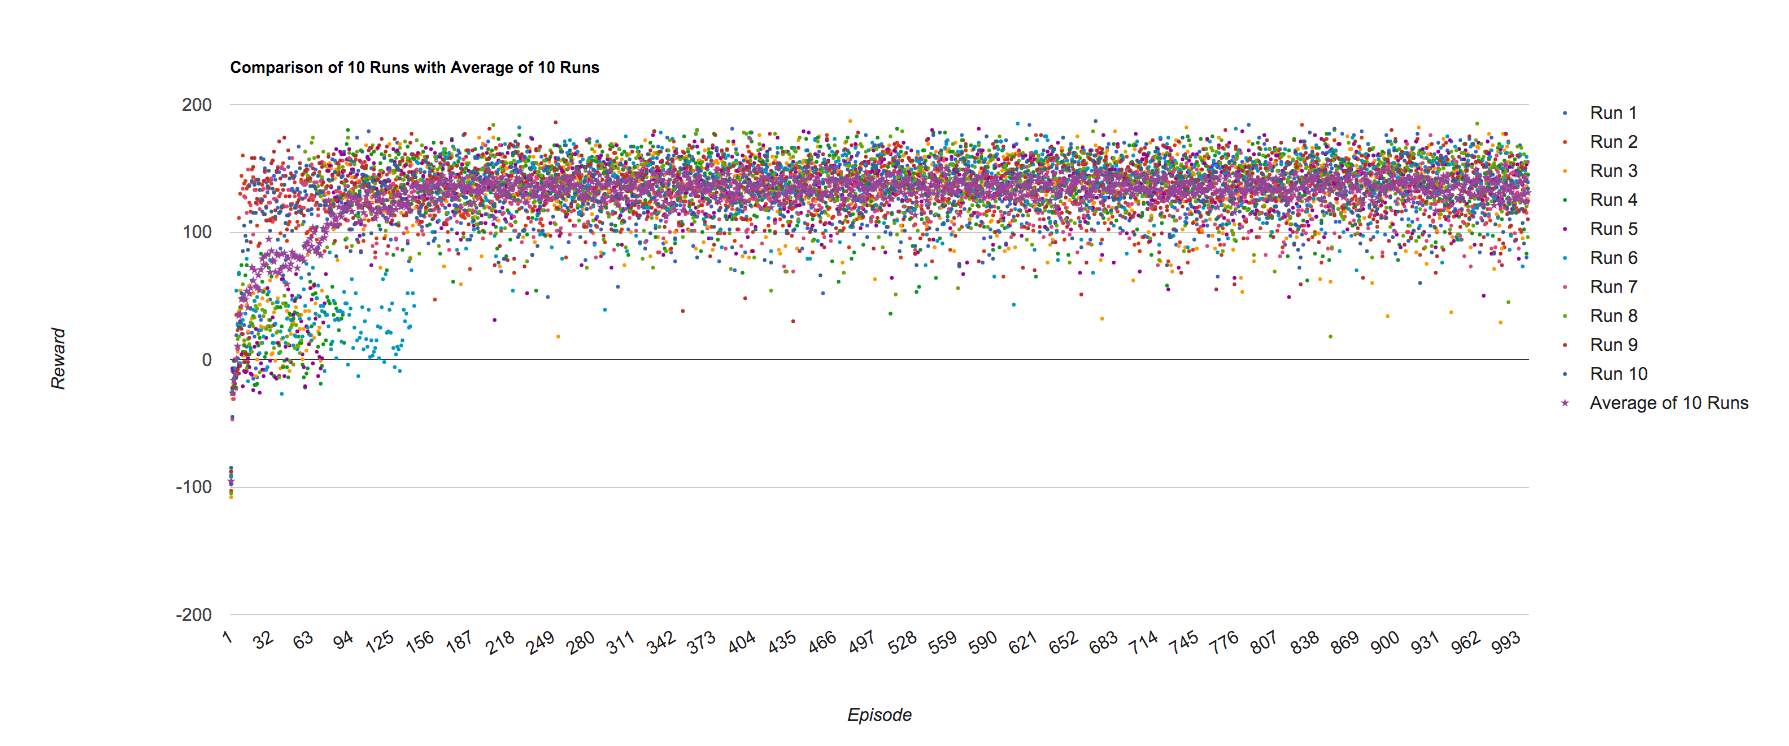
\includegraphics[scale=.25]{regular} \\
                It can be seen that with learning, the agent drastically improves it performance. As shown with the "Average" plot, the robot is increasing in performance and remaining in the positive reward zone as well.\\
                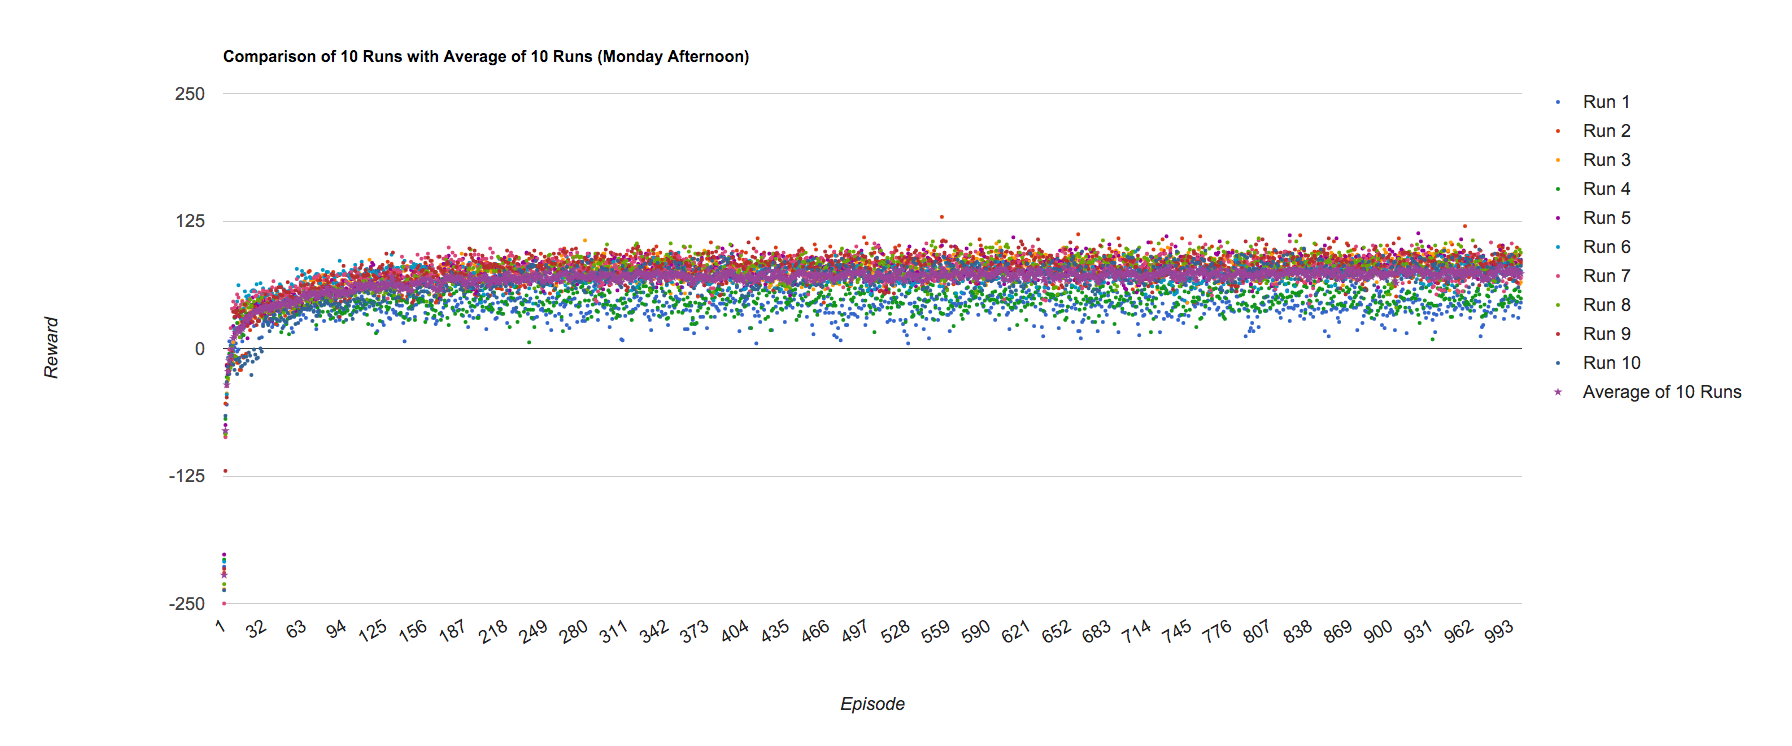
\includegraphics[scale=.25]{mmafter}\\
                The afternoon simulation has a much smaller steady state reward and in addition has a much smaller spread in the steady state reward when compared to the default Monday morning simulation. For all following simulations, similar results were witnessed in both the morning and afternoon simulations.
                \item 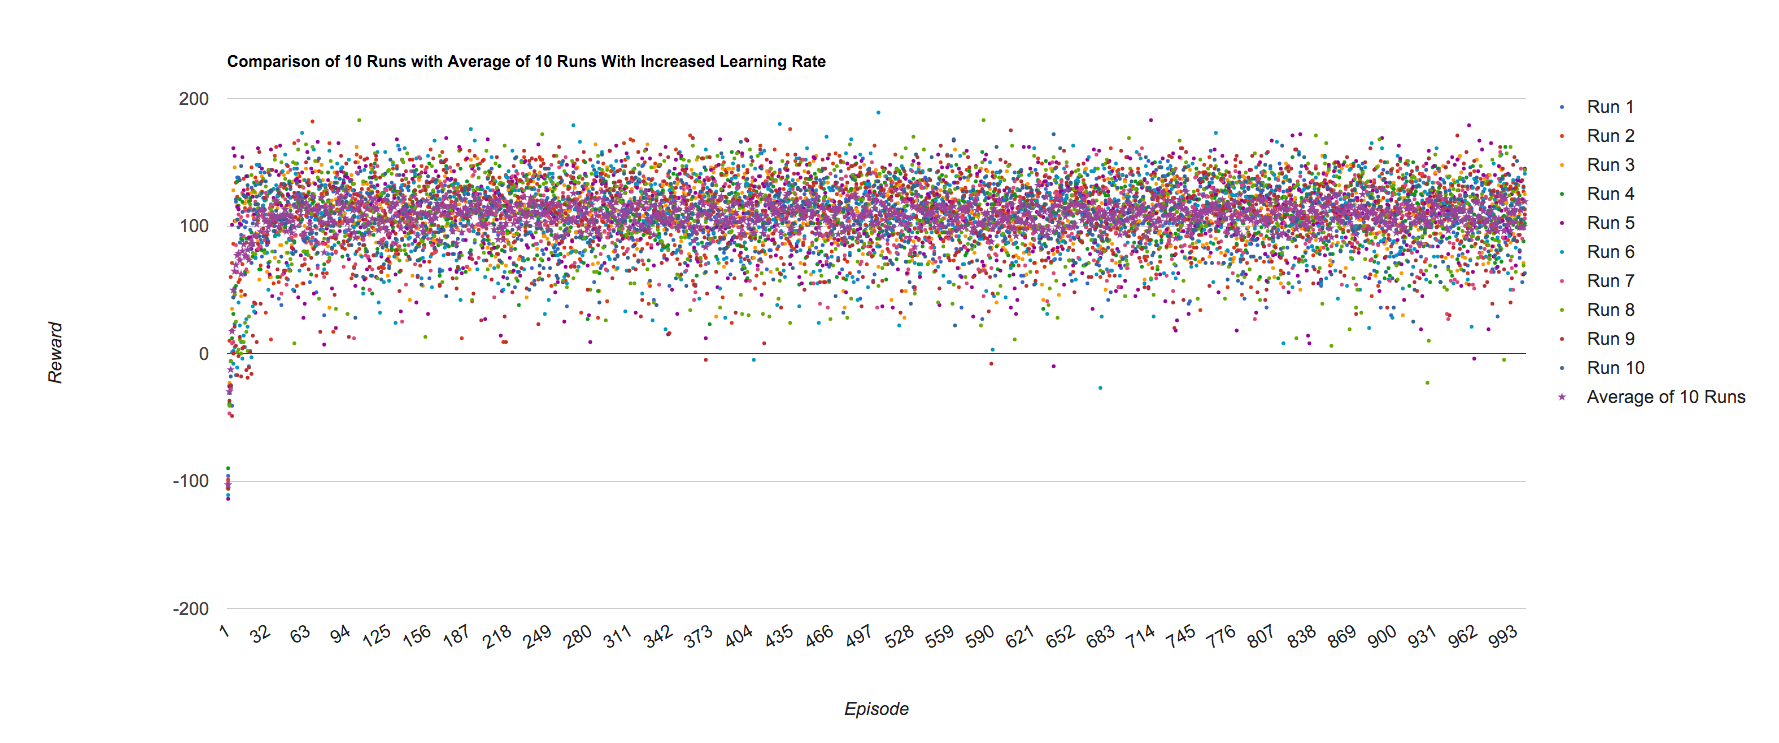
\includegraphics[scale=.25]{increased_rate} \\
                By increasing the learning rate, it can be seen that the initial learning slope is greatly increased, causing the agent to learn faster than the initial learning value.
                \item 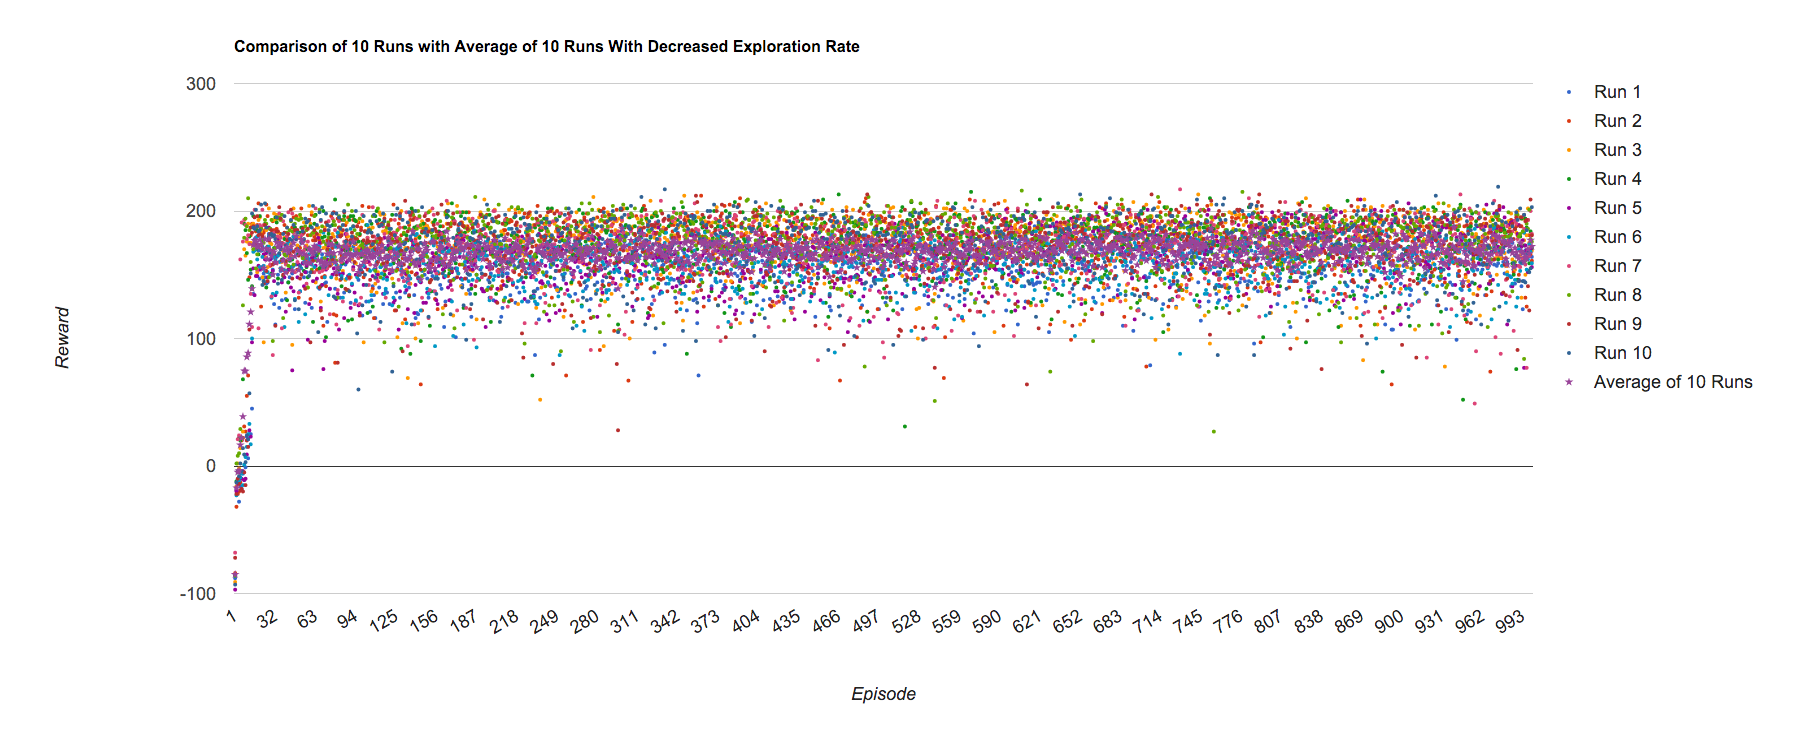
\includegraphics[scale=.25]{decrased_exp} \\
                The decrease in learning rate does not cause a significant change between the increase in learning rate plot. The only noticeable change is that, compared to the increased learning rate graph, this plot has a much more linear initial slope, perhaps due to the fact that the agent is more likely to choose the best option for movement. However, the initial learning slope for the agent is much steeper than the default values for the agent. 
                $\infty$
            \end{enumerate}
    \end{enumerate}
\end{document}